\documentclass[11pt, oneside]{article} 
\usepackage{geometry}
\geometry{letterpaper} 
\usepackage{graphicx}
	
\usepackage{amssymb}
\usepackage{amsmath}
\usepackage{parskip}
\usepackage{color}
\usepackage{hyperref}

\graphicspath{{/Users/telliott_admin/Dropbox/Tex/png/}}
% \begin{center} 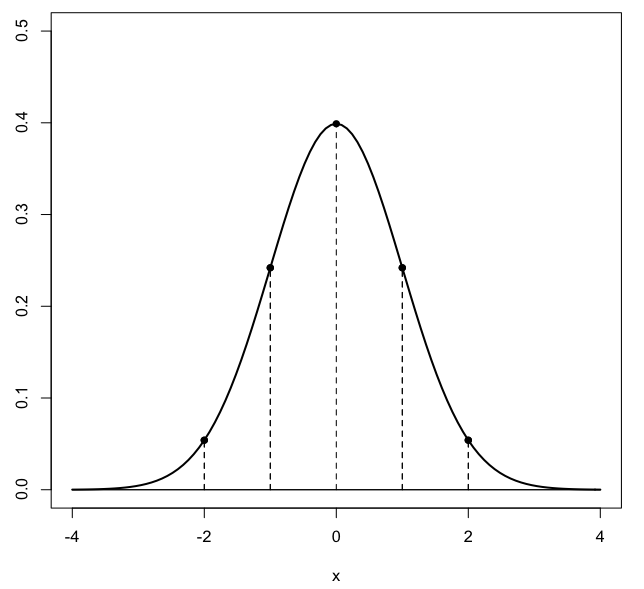
\includegraphics [scale=0.4] {gauss3.png} \end{center}

\title{Cycloid}
\date{}

\begin{document}
\maketitle
\Large

We imagine a bicycle with one tire marked at a particular point on the rim, say with fluorescent paint or a small light.  Time starts at $t = 0$ with that point $P$ in contact with the $x$ axis at $(0,0)$.  Then we start rolling the bike.  As the tire rotates our fixed point $P$ on the rim traces a curve
\begin{center} 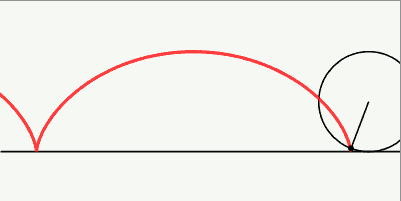
\includegraphics [scale=0.6] {cycloid.png} \end{center}

We want to find equations that give the position of the point $P$ as a function of time.  We will parametrize the curve, yielding parametric equations $x(t)$, $y(t)$.

The second diagram  shows the angle through which the wheel has turned as $\theta$, but we will use $t$ for $\theta$ here.  

\begin{center} 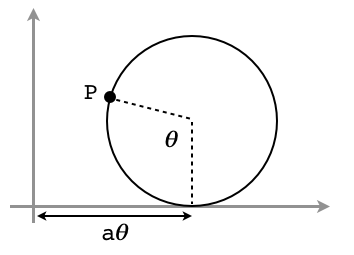
\includegraphics [scale=0.5] {cycloid2.png} \end{center}
The $x$ displacement of the vertical straight down from the center of the tire is just $at$, where $a$ is the radius of the wheel, it is equal to the arc on the circumference of the wheel from the point which is currently in contact with the ground, going around up to $P$.

It is reasonably easy to derive the desired parametric equations, using vectors, especially once you know the answer.  For $x$, we have the vector that goes from $(0,0)$ to the contact point with the ground.  As indicated in the figure, that is $at$.  

We need to subtract the distance $a \ sin\ t$ from that.  Basically the rationale is that the motion is a standard parametric circle which has been rotated by $90$ degrees clockwise and then inverted.  The rotation changes cosine to sine, and the inversion the subtraction.

It's easier to see for $t < \pi/2$, but it is true always.  Check some other values of $t$ like $\pi$ or $3\pi/2$ to confirm.  This is the usual circular motion.

For $y$, we have a constant factor of $a$ above the $x$ axis, then the additional displacement is $-a \ cos \ t$.  So for $t=0$ we have the additional displacement is -a (we were on the ground), for $t=\pi/2$ it is zero, and for $t=\pi$ it is plus $a$ for a total of $2a$.

The parametric equations are then
\[ x(t) = at - a \sin t \]
\[ y(t) = a - a \cos t \]
Taking derivatives:
\[ x'(t) = a - a \cos t \]
\[ y'(t) = a \sin t  \]

The derivation above did a little mental gymnastics with the circle, flipping it and setting $t=0$ when the point is at the bottom.  As an alternative, leave the circle in its usual orientation, with an angle $s$ to the positive $x$ axis.

It can be seen easily that $s$ and $t$ are related by the equation 
\[ s = 3\pi/2 - t \]

The vector from the center of the circle to the point on the edge is just the standard one for a point on a circle of radius $a$:
\[ a \ \langle \cos s, \sin s  \rangle \]
For the $x$ component:
\[ \cos s = \cos 3 \pi / 2 - t \]
\[ = \cos 3 \pi / 2  \cos t + \sin 3 \pi / 2 \sin t \]
Recall that $\cos 3 \pi / 2 = 0$ and $\sin 3 \pi / 2 = -1$ so
\[ \cos s = - \sin t \]
And for the $y$ component
\[ \sin s = \sin 3 \pi / 2 - t \]
\[ = \sin 3 \pi / 2 \cos t - \sin t \cos  3 \pi / 2 \]
\[ = - \cos t \]
The vector is then
\[ a \ \langle \cos s, \sin s  \rangle = a \ \langle -\sin t, -\cos t  \rangle \]

In addition, we have to add another vector, one extending from the origin to the center of the wheel.  The $y$ component is constant, it is just $a$.  The $x$-component is the distance the wheel has traveled from its initial position (the distance between the origin and the point of contact with the $x$-axis, which is $at$, shown as $a \theta$ in the figure).

Hence the vector to the point is:
\[ a \ \langle -\sin t, -\cos t  \rangle + \langle at, a \rangle \]
\[ a \ \langle t - \sin t, 1 - \cos t \rangle \]

which matches what we had before.

\subsection*{Arc length}
We wish to determine the arc length and area under the curve for one complete revolution of the wheel.

We want to use a slightly different version of the usual formula for arc length

\[ ds^2 = dx^2 + dy^2 \]
\[ (\frac{ds}{dt})^2 = (\frac{dx}{dt})^2 + (\frac{dy}{dt})^2 \]
\[ ds = \sqrt{(\frac{dx}{dt})^2 + (\frac{dy}{dt})^2} \ dt \]
\[ = \sqrt{(a - a \cos\ t)^2 + (a \sin\ t)^2} \ dt  \]
This expands to
\[ a \sqrt{1 - 2 \cos\ t + \cos^2t + \sin^2t } \ dt \]
\[ =  a \sqrt{2 - 2 \cos \ t} \ dt\] 
The length is
\[ L = \int_0^{2\pi} a \sqrt{2 - 2 \cos \ t} \ dt\]
\[ = a \sqrt{2} \ \int_0^{2\pi} \sqrt{1 - \cos \ t} \ dt\]

\subsection*{double angle}

\[ \cos (s-t) = \cos s \cos t + \sin s \sin \ t \]
(check:  if $s=t$ then $\cos 0 = 1$, which is correct).

So
\[ \cos (s+t) = \cos s \cos t - \sin s \sin \ t \]
Let $s = t$ and $u = 2s$, then
\[ \cos 2s = \cos u = \cos^2 \ (\frac{u}{2}) - \sin^2 \ (\frac{u}{2}) \]
\[ \cos u = 1 - \sin^2 \ (\frac{u}{2}) - \sin^2 \ (\frac{u}{2}) \]
\[ 2 \sin^2 \ (\frac{u}{2}) = 1 - \cos u \]
$u$ is just a dummy variable, so we can switch back to $t$
\[ 2 \sin^2 \ (\frac{t}{2}) = 1 - \cos t \]

\subsection*{finishing up}
We have that 
\[ L = a \sqrt{2} \ \int_0^{2\pi} \sqrt{1 - \cos \ t} \ dt\]
And
\[ 1 - \cos t = 2 \sin^2(\frac{t}{2}) \]
\[ \sqrt{1 - \cos t} = \sqrt{2} \sin(\frac{t}{2}) \]
So
\[ L = a \sqrt{2} \ \int_0^{2\pi} \sqrt{2} \sin \ (\frac{t}{2}) \ dt\]
\[  = 2a  \ \int_0^{2\pi} \sin \ (\frac{t}{2}) \ dt\]
\[ = 2a \ (-2) \cos \ (\frac{t}{2})\ \bigg |_0^{2\pi} \]
\[ = -4a \ (\cos \ \pi - \cos \ 0) \]
\[ = -4a \ (-1 - 1) = 8a\]
A simple answer to the problem.

\subsection*{Area under the arc}
We want
\[ A = \int_{t=0}^{t=2\pi} y \ dx \]
\[ = \int_{t=0}^{t=2\pi} (a - a \cos\ t) (a - a \cos\ t) \ dt \]
\[ a^2\int_{t=0}^{t=2\pi} (1 - \cos\ t) (1 - \cos\ t) \ dt \]
\[ a^2\int_{t=0}^{t=2\pi} (1 - 2 \cos\ t + \cos^2\ t) \ dt \]
If you don't remember the result for $\int \cos^2 t \ dt$, you can go back to the double angle formula above and convert from $\sin^2$ to $\cos^2$.  Otherwise recall it and write:
\[ A = a^2 ( t - 2 \sin \ t + \frac{1}{2}t + \frac{1}{4} \sin 2t ) \ \bigg|_0^{2\pi} \]
\[ a^2 ( 2\pi - 0 + \pi + 0 - 0 + 0 - 0 - 0    ) = 3\pi a^2 \]
Also a very simple answer.

\end{document}